
\documentclass{article}
\usepackage[utf8]{inputenc}
\usepackage{listings}
\usepackage{amsmath}
\usepackage{amssymb}
\usepackage{mathtools}
\usepackage{amsfonts}
\usepackage[margin=20mm]{geometry}
\usepackage{fancyvrb}
\usepackage{qtree}
\usepackage{float}
\usepackage{graphicx}
\graphicspath{ {./} }
\usepackage{textcomp}
\usepackage[linguistics]{forest}
\restylefloat{table}
\newcommand{\f}[2]{f_{#1}(#2)}
\newcommand{\code}[1]{\texttt{#1}}
\DeclarePairedDelimiter{\ceil}{\lceil}{\rceil}
\DeclarePairedDelimiter\set\{\}
\DeclarePairedDelimiter{\parens}{\lparen}{\rparen}
\title{HW1 Wet}
\date{}
\begin{document}
\maketitle
\section*{Description of the Data Structure:}
    \begin{figure}[h]
    \caption{Visual Representation of the Data Structure}
    \centering
    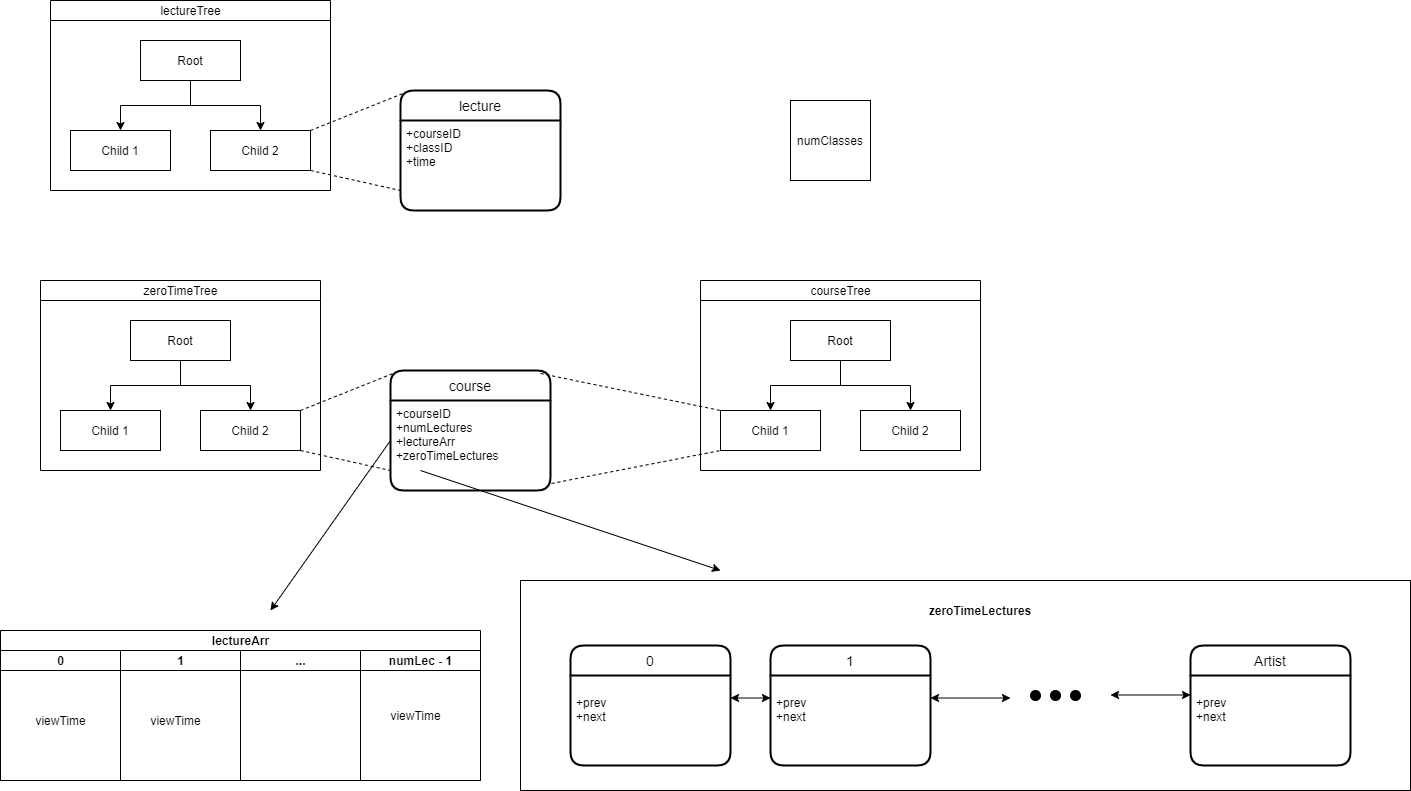
\includegraphics[width=\textwidth]{ds_layout}
    \end{figure}
    The data structure contains three AVL trees that have additional fields of \texttt{min} and \texttt{max}
    to allow for in-order and post-order traversal of $k$ nodes in the tree in $O(k)$ time:
    \begin{itemize}
        \item \code{lectureTree}: Contains all the lectures of all the courses in the system. Each lecture in 
                the tree maintains exactly three pieces of information: The ID of the lecture, the ID of the 
                course in which the lecture is given, and the total watch time for the lecture. 
                Together, these three pieces of information form the key by which the lectures in the tree are sorted 
                (according to the sort order stipulated in \code{getMostViewedClasses}): By descending view time,
                then by ascending course ID and then by ascending lecture ID.
        \item \code{courseTree}: Contains all the courses in the system. Is sorted by course ID. 
        \item \code{zeroTimeTree}: Contains all the courses in the system that have at least one lecture 
                with a watch time of zero. Is also sorted by course ID. 

    \end{itemize}
    The courses in both \code{courseTree} and \code{zeroTimeTree} are represented by objects with
    which contain four fields:
    \begin{itemize}
        \item \texttt{courseID}: The ID of the course
        \item \texttt{numLectures}: The number of lectures in the course
        \item \texttt{lectureArr}: An array conataining a number  of cells equal to the 
                the number of lectures in the course. The index of each cell is the ID of the 
                relevant lecture and the contents of the cell is that lecture's watch time.
        \item \texttt{zeroTimeLectures}: An array similar to \texttt{lectureArr} except that it holds
                only the lectures of the course that have a watch time of zero. In addition, it has features
                of a doubly linked list, meaning that every cell has \texttt{prev} and \texttt{next} fields
                that hold the indices of the previous and next non-empty cell. This means thst \texttt{zeroTimeLectures}
                has both the capability of adressing a cell in $O(1)$ time as an array would, as well as the
                the cabaility of traversing $k$ non-empty cells in $O(k)$ time as a doubly-linked would
                be able to do.
    \end{itemize}
    In addition, the structure maintains a variable \texttt{numClasses} which tracks the total number of 
    lectures of all the courses in the system at any given moment.
\section*{Space Complexity of the Data Structure}
    At any moment, there is at most three copies of every lecture in the system ($3m$) - two in 
    the course object (one being in the \texttt{lectureArr} and the other in \texttt{zeroTimeLectures} of the course)
    in \texttt{courseTree}, and if the watch time of the lecture is zero than two more in the course in
    \texttt{zeroTimeTree} and otherwise, one copy in \texttt{lectureTree}.
    Furthermore, there is always at most two copies of every course in the system ($2n$): one in 
    \texttt{courseTree}, and in the case that the course has a lecture with a view time equal to zero, 
    an additional copy in \texttt{zeroTimeTree}.
    Therefore, the total space complexity of the structure is $O(n+m)$.



\section*{Implementation of the Data Structure}
    For all the function that receive parameters, the validity of those parameters is checked. In the case that one
    or more of the parameters is invlid, \texttt{INVALID\_INPUT} is returned. This check always only takes a constant 
    amount of time to perform ($O(1)$). Additonally, in all the functions that have a return value, in the case
    that the function successfuly finnished, it returns \texttt{SUCCESS}, which also only takes $O(1)$ time.
    \subsection*{Init}
        \texttt{lectureTree}, \texttt{courseTree}, and \texttt{zeroTimeTree} are all initiallized (as empty), 
        which each take $O(1)$ time. In addition \texttt{numCLasses} is initiallized to zero ($O(1)$ time).
        Therefore, the total time complexity for \texttt{Init} is $O(1)$.
    \subsection*{AddCourse}
        \begin{enumerate}
            \item First, we search \texttt{courseTree} to see if the course that is being requested to be added
                is already in the system. If this is the case, we return \texttt{FAILURE}. The size of
                \texttt{courseTree} at any given moment is exactly the $n$, the number of courses in the 
                system, and therefore this action is a search on a AVL tree of size n, which according 
                to the lecture takes $O(\log(n))$ time.
            \item If the course is not yet in the system, we create a course object for the course to
                be inserted. This consists of initializing \texttt{lectureArr}, an array of zeroes of
                size $m=\texttt{numOfClasses}$ which therefore takes $O(m)$ time, initialization of 
                \texttt{zeroTimeLectures} also to a size of $m$ which also takes $O(m)$ time, and initialization
                of \texttt{numLectures} to $m$ ($O(1)$).
            \item Next, the course object created in the previous step is inserted into \texttt{courseTree} and
                into \texttt{zeroTimeTree}, each being an insertion into an AVL tree of size $n$, and therefore each 
                taking $O(\log(n))$.
            \item Finally, \texttt{numOfClasses} is added to \texttt{numClasses} ($O(1)$).
        \end{enumerate}
    Therefore in total, \texttt{AddCourse} is of $O(\log(n))+2\cdot O(m)+O(1)+2\cdot O(\log(n))+O(1))=O(\log(n)+m)$ time complexity.
    \subsection*{RemoveCourse}
        \begin{enumerate}
            \item First, we search \texttt{courseTree} to see if the course that is being requested to be removed
                is actually in the system. If this is not the case, we return \texttt{FAILURE}. The size of
                \texttt{courseTree} at any given moment is exactly the $n$, the number of courses in the 
                system, and therefore this action is a search on a AVL tree of size n, which according 
                to the lecture takes $O(\log(n))$ time.
            \item If the course is indeed in the system, for each of its lectures we delete the matching 
                lecture from \texttt{lectureTree} (if the lecture is in that tree, meaning if it has a 
                watch time that is greater than zero). At worst this will take $O(m\cdot \log(M))$ time, if 
                all $m$ of the course's lectures have greater than zero watch time, since we are doing $m$ removals
                from an AVL tree of maximal size $M$ (because at most it cpontains all the lectures in the system)
                 and then deleting each lecture which was removed, each being of $O(1)$ size.
            \item Next, if the course has lectures of zero watch time, we delete the course from the 
                \texttt{zeroTimeTree}. This involves removal from an AVL tree of at most $n$ (because the 
                tree at most contains all the courses in the system) which therefore takes $O(\log (n)$ time, and 
                then deletion of the course that was removed ($O(m)$ each for deleting \texttt{lectureArr} and 
                \texttt{zeroTimeLectures} and $O(1)$ each for deleting \texttt{courseID} and \texttt{numLectures}).
            \item In an identical fashion, the course is removed from \texttt{courseTree}.
            \item Finally, the number of lectures that were in the course that
            was removed is subtracted from \texttt{numClasses} ($O(1)$).
        \end{enumerate}
    Therefore in total, \texttt{RemoveCourse} is of 
     \begin{align*}
         &O(\log(n))+O(m\cdot \log(M))\cdot O(1)+2\cdot (O(\log(n))+2\cdot O(m)+2\cdot O(1))+O(1)\\
         &=O(\log(M))+O(m\cdot \log(M))\cdot O(1)+2\cdot (O(\log(M))+2\cdot O(m)+2\cdot O(1))+O(1) && (\text{we can assume } n < M)\\
         &= O(m\log(M)) && (m=O(m\log(M)))
     \end{align*}
     time complexity.
    \subsection*{WatchClass}
        \begin{enumerate}
            \item First, we search \texttt{courseTree} to see if the course that is supplied 
                is actually in the system. If this is the case, but the \texttt{classID} supplied
                is not one of the classes of \texttt{courseID}, than we return \texttt{INVALID\_INPUT}.
                As previously shown, the search for the course in the tree takes $O(\log(n))$, and the further
                validation of the class being a valid class of the course requires merely checking if 
                $\texttt{classID}+1>\texttt{numLectures}$ which is only $O(1)$ time.
            \item Next, we search \texttt{courseTree} to see if the course that is supplied 
                is actually in the system. If this is the not the case than we return \texttt{FAILURE}.
                As previously shown, the search for the course in the tree takes $O(\log(n))$.
            \item Next, we check what the watch time of \texttt{classID} is by getting the course from 
                \texttt{courseTree} and checking \texttt{lectureArr}[\texttt{classID}] ($O(\log(n))+O(1)$).
                \begin{itemize}
                    \item If the watch time is zero, we remove \texttt{classID} from \texttt{zeroTimeLectures}
                    in the same course object. This invloves marking the applicable cell in \texttt{zeroTimeLectures}
                    as empty and then adjusting the \texttt{prev} and  \texttt{next} field in the adjacent cells apporpraitely
                    as is done in a doubly linked list (which is a finite amount of constant time complexity actions: $O(1)$).
                    If after this removal \texttt{zeroTimeLectures} is empty, then the course is removed from \texttt{zeroTimeTree}
                    ($O(\log(n))$). 
                    \item If the watch time is not zero, then the matching lecture is removed from \texttt{lectureTree} ($O(\log(M))$).
                \end{itemize}
            \item Next, the \texttt{time} that was supplied to \texttt{WatchClass} is added to the \texttt{time}
                 of the lecture that was removed in the previos step ($O(1)$). The lecture is then re-inserted
                 into \texttt{lectureTree} ($O(\log(M))$).
            \item Finally, the \texttt{time} that was supplied to \texttt{WatchClass} is added to the 
                \texttt{courseArr}[\texttt{classID}] in the course in \texttt{courseTree} ($O(\log(n))+O(1)$).
        \end{enumerate}
    Therefore in total, \texttt{WatchClass} is of 
     \begin{align*}
         &5\cdot O(\log(n))+2\cdot O(\log(M))+5\cdot O(1)\\
         &=5\cdot O(\log(M))+2\cdot O(\log(M))+5\cdot O(1) && (\text{we can assume } n < M)\\
         &=O(\log(M))\\
         &=O(\log(M)+t)
     \end{align*}
     time complexity.
    \subsection*{TimeViewed}
        \begin{enumerate}
            \item First, we search \texttt{courseTree} to see if the course that is supplied 
                is actually in the system. If this is the case, but the \texttt{classID} supplied
                is not one of the classes of \texttt{courseID}, than we return \texttt{INVALID\_INPUT}.
                As previously shown, the search for the course in the tree takes $O(\log(n))$, and the further
                validation of the class being a valid class of the course requires merely checking if 
                $\texttt{classID}+1>\texttt{numLectures}$ which is only $O(1)$ time.
            \item Next, we search \texttt{courseTree} to see if the course that is supplied 
                is actually in the system. If this is the not the case than we return \texttt{FAILURE}.
                As previously shown, the search for the course in the tree takes $O(\log(n))$.
            \item Finally, \texttt{courseArr}[\texttt{classID}] in the course in \texttt{courseTree}
            is coppied into \texttt{timeViewed} ($O(\log(n))+O(1)$).
        \end{enumerate}
    Therefore in total, \texttt{TimeViewed} is of 
     \begin{align*}
         &3\cdot O(\log(n))+2\cdot O(1)\\
         &=O(\log(n))
     \end{align*}
     time complexity.
    \subsection*{GetMostViewedClasses}
        \begin{enumerate}
            \item First, we check if $\texttt{numOfClasses}>\texttt{numCLasses}$.
                 If so, then we return \texttt{FAILURE} ($O(1)$).
            \item Otherwise, we perform an in-order traversal of \texttt{numOfClasses} number of lectures 
                in \texttt{lectureTree} beginning with the one with the highest key (with the highest view time).
                At each lecture that is stopped at, its course ID is coppied into the next cell in \texttt{courses},
                and its class ID is coppied into the next cell in \texttt{classes}.
            \item If \texttt{numOfClasses} is greater than the number of lectures in \texttt{lectureTree}, than the following
                procedure is followed for the remaining number of \texttt{numOfClasses} times, beginning with the course
                with the lowest \texttt{courseID} in \texttt{zeroTimesTree}, for each course in an in-order traversal:
                \begin{enumerate}
                    \item For each cell that is not empty in \texttt{zeroTimeLectures}, copy the course ID of the current
                        course we are in into \texttt{courses} and copy the current index of \texttt{zeroTimeLectures}
                        into \texttt{classes}.
                \end{enumerate}

        \end{enumerate}
    At every step, either an in-order traversal is being performed on an AVL tree or a linear traversal of 
    a linked list. The actions peformed at every stop are a copy of two pieces of data, which each take
    $O(1)$ time to perform. The total number of steps is $m=\texttt{numOfClasses}$. Therefore in total, \texttt{getMostViewedClasses} is of 
     \begin{align*}
         &m\cdot O(1)\\
         &=O(m)
     \end{align*}
     time complexity.
    \subsection*{Quit}
        \begin{enumerate}
            \item First, we delete every lecture in \texttt{lectureTree}. The number of lectures in \texttt{lectureTree}
                is at most equal to the total number of lectures in the system, $m$. Therefore this takes $O(m)$ time
                to complete.
            \item Next, we delete every lecture held in every course in \texttt{zeroTimeTree},
                as well as all the courses themselves in the tree. Every lecture in the system can appear at most 
                twice in \texttt{zeroTimeTree}: once in a \texttt{lectureArr} and once in a \texttt{zeroTimeLectures}.
                Therefore, the total number of lectures in the tree is at most equal to the total number of lectures in the system, $m$,
                multiplied by two: $2m$, and the total number of courses
                in \texttt{zeroTimeTree} is at most equal to the total number of courses in the system, $n$.
                Therefore it takes $O(2m+n)=O(m+n)$ time to delete \texttt{zeroTimeTree}.
            \item In the identitcal way that we deleted \texttt{zeroTimeTree}, we delete \texttt{courseTree}.
                For the identical reasoning, it also takes $O(m+n)$ time.
        \end{enumerate}
    Therefore in total, \texttt{Quit} is of 
     \begin{align*}
         &O(m)+2\cdot O(m+n)\\
         &=O(m+n)
     \end{align*}
     time complexity.
\end{document}